\section{Cenário}
\label{sec:cenario}
Nesse cenário, cada dispositivo da casa (veículo de carga terrestre, elevador, garra mecânica) é disponibilizado como um serviço Web RESTFul (seção \ref{subsec:dispositivosWeb}). O HS disponibiliza o serviço ``Levar compras'' através de uma API RESTFul, e este á acionado por um \textit{smartphone}. O serviço quando acionado leva as compras colocadas num veículo, por um humano, até as proximidades do elevador de carga, dado esse momento a garra mecânica coloca as compras no elevador e este então completa o serviço de transporte ``Levar compras''.


Diante do crescente cenário da IoT, diversos disposi
falar dos métodos de detecção utilizadasos n ainteracao entre servicos e dizer que as abordagens propostas não considera o comportamento do dispositivo, ou seja, apesar do feature cumprir sua funcionalidad corretmante, o comportamento desta feature junto com as outras levam a resultados não esperados pelo sistema.

Para verificar a vericidade da hipótese...
-disponibilização dos serviços como serviços Web RESTFul
-é stateful / assíncrono
-realizar experimentos para observar a interação entre os serviços
-
\section{Conjunto de dados}
\label{sec:dataset}
\section{Metodologia}
**Coloca o desvio padrão tb na comparação das medidas.
\begin{figure}[!htb] \centering 
  \centering
  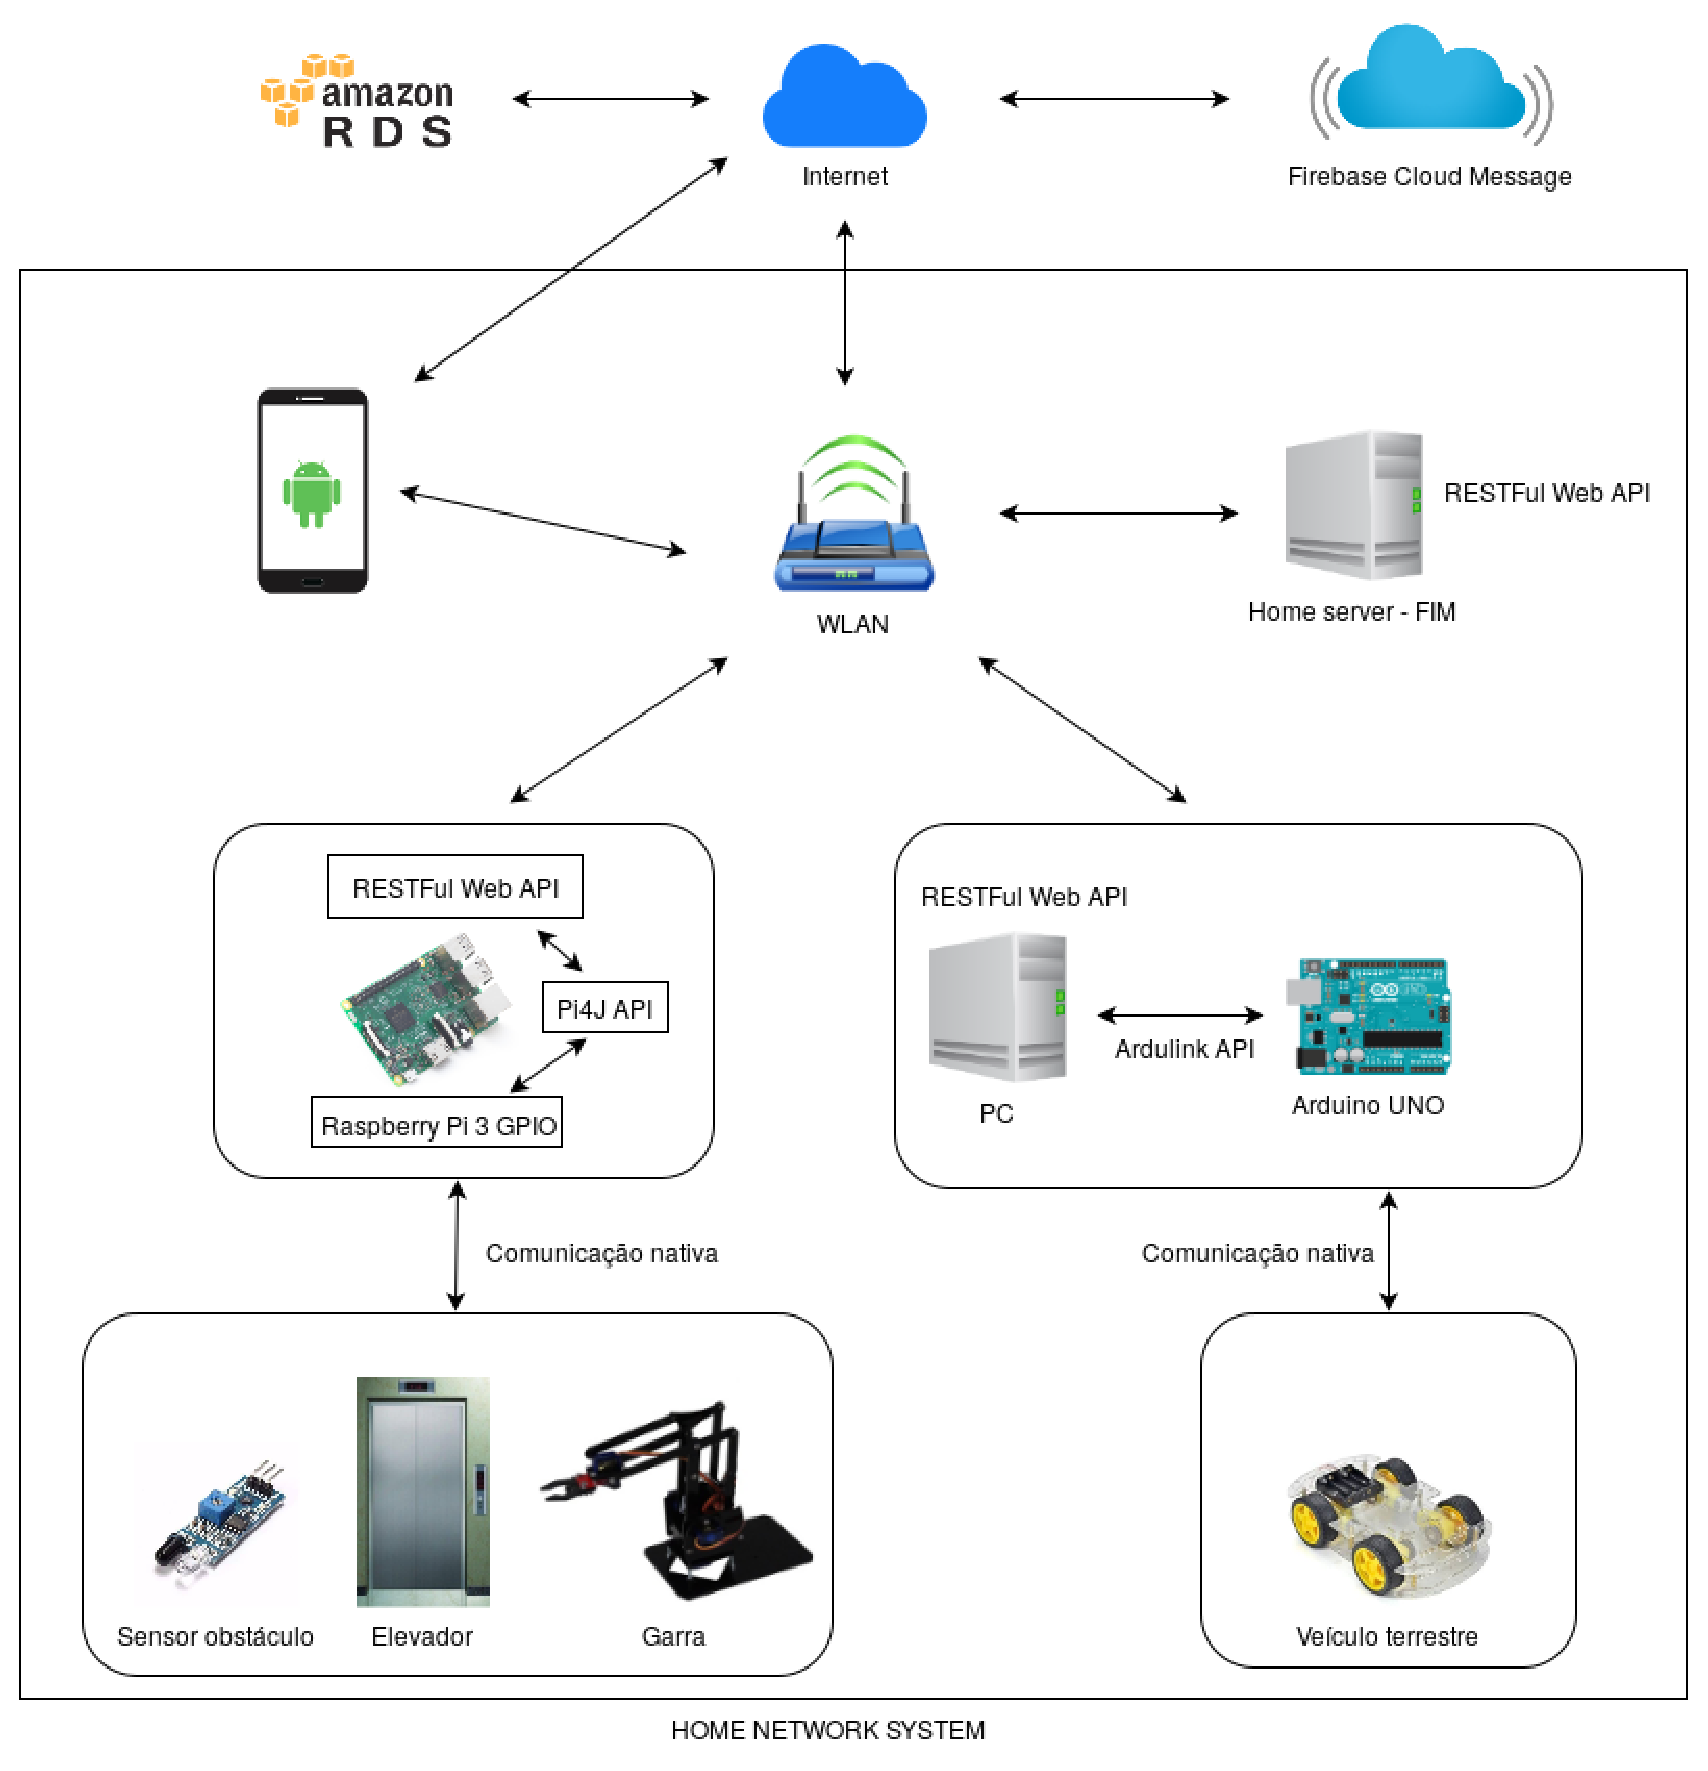
\includegraphics[width=0.8\columnwidth]{cenario} 
  \caption{Modelo do HNS utilizado neste trabalho.} 
  \label{fig:hnsworkmodel}
\end{figure}


**ver se dar tempo de gerar curva roc(verifdicar o motivo da roc, é viavel para este cenário) e precision e recall dos resultados dos 3 modelos**

MOTIVO:
escolher os melhores parametros para o modelo em questão, neste caso, rede neural.

 machine learning and statistics, feature selection, also known as variable selection, attribute selection or variable subset selection, is the process of selecting a subset of relevant features (variables, predictors) for use in model construction. Feature selection techniques are used for three reasons:

        simplification of models to make them easier to interpret by researchers/users,[1]
        shorter training times,
        enhanced generalization by reducing overfitting[2](formally, reduction of variance[1])

Procedimentos utilizados - experimento:
-gera uma plotMatriz dos dados do dataset
-verifica quais dados poderiam ser melhor separados por uma curva(par a par)

-neste caso, visualmente são esse abaixo:
t_num_width e t_num_diameter
(quem não tem width, tem diameter e vice e versa)
t_num_mass e t_num_width

-testa com alguma combinação distinta dos parâmetros acima
t_num_width, t_num_mass, t_num_diameter 

The limitation to just one layer of hidden neurons is justified by the fact that one hidden layer is enough to approximate any continuous function (6,7).\cite{Pasini:2015}

-Verifica a generalização utilizando técnicas estaitisticas, tais como, stratifyed-k-crossvalidation e/ou randomized-holdout

-escolhe o melhor modelo baseado no que você quer do modelo, neste caso o que tiver melhor recall, seguido de accuracy. POIS É MELHOR ERRAR DIZENDO QUE É, DO QUE ERRAR DIZENDO QUE NÃO É.

-gera um classificador com todo o dataset verificado na etapa anterior.
-testa esse classificador com um dataset distinto do anterior.
-DEMONSTRA OS RESULTADOS E COMPARA COM OS TESTES ANTERIORES.
\section{Resultados}
-modelo de clasificado bom para o cenário
-implantar o classificador no sistema